\clearpage
\subsection{Comparison between 1D and 2D finite element discretization}
\begin{table}[]
\centerline{\bf 1D and 2D Comparison for Finite Element and Multigrid }\medskip
\centering
\begin{tabular}{ p{7cm}<{\centering}|p{7cm}<{\centering}}
\hline
%\smallskip 
   $1D: \Omega=(0, 1)$      \smallskip &    $2D: \Omega=(0, 1)\times (0, 1)$     
%\smallskip 
  \\\hline
 $\begin{cases}
 -u''=f&x\in \Omega\\
 u(0)=u(1)=0&
 \end{cases}$        &     
 $\begin{cases}
 -\triangle u=f&x\in \Omega\\
 u=0&x\in \partial \Omega
 \end{cases}$       
 \\\hline
  \multicolumn{2}{c}{$\displaystyle u=\argmin_{v\in V}   J(v)$}   
 \\\hline
  $\displaystyle J(v)={1\over 2}\int_0^1  |v'|^2dx - \int_0^1  fv dx $
  &     $\displaystyle J(v)={1\over 2}\int_\Omega  |\nabla v|^2dx - \int_\Omega fv
  dx $      
 \\\hline
 \multicolumn{2}{c}{$V=\{v: \Omega\rightarrow \mathbb{R} \mbox{ is continuous and piecewise smooth, } v|_{\partial \Omega}=0\}$}
 \\\hline 
  \multicolumn{2}{c}{FE space: $V_h=\{v_h\in V, v_h \mbox{ is piecewise linear w.r.t. } \mathcal{T}_h\}$}  
\\\hline
\begin{minipage}{0.5\textwidth}\centering
      	\includegraphics[width=4cm]{figures/grid1d.png}
   	 \end{minipage}  
    	&  
	\begin{minipage}{0.2\textwidth}\centering
      	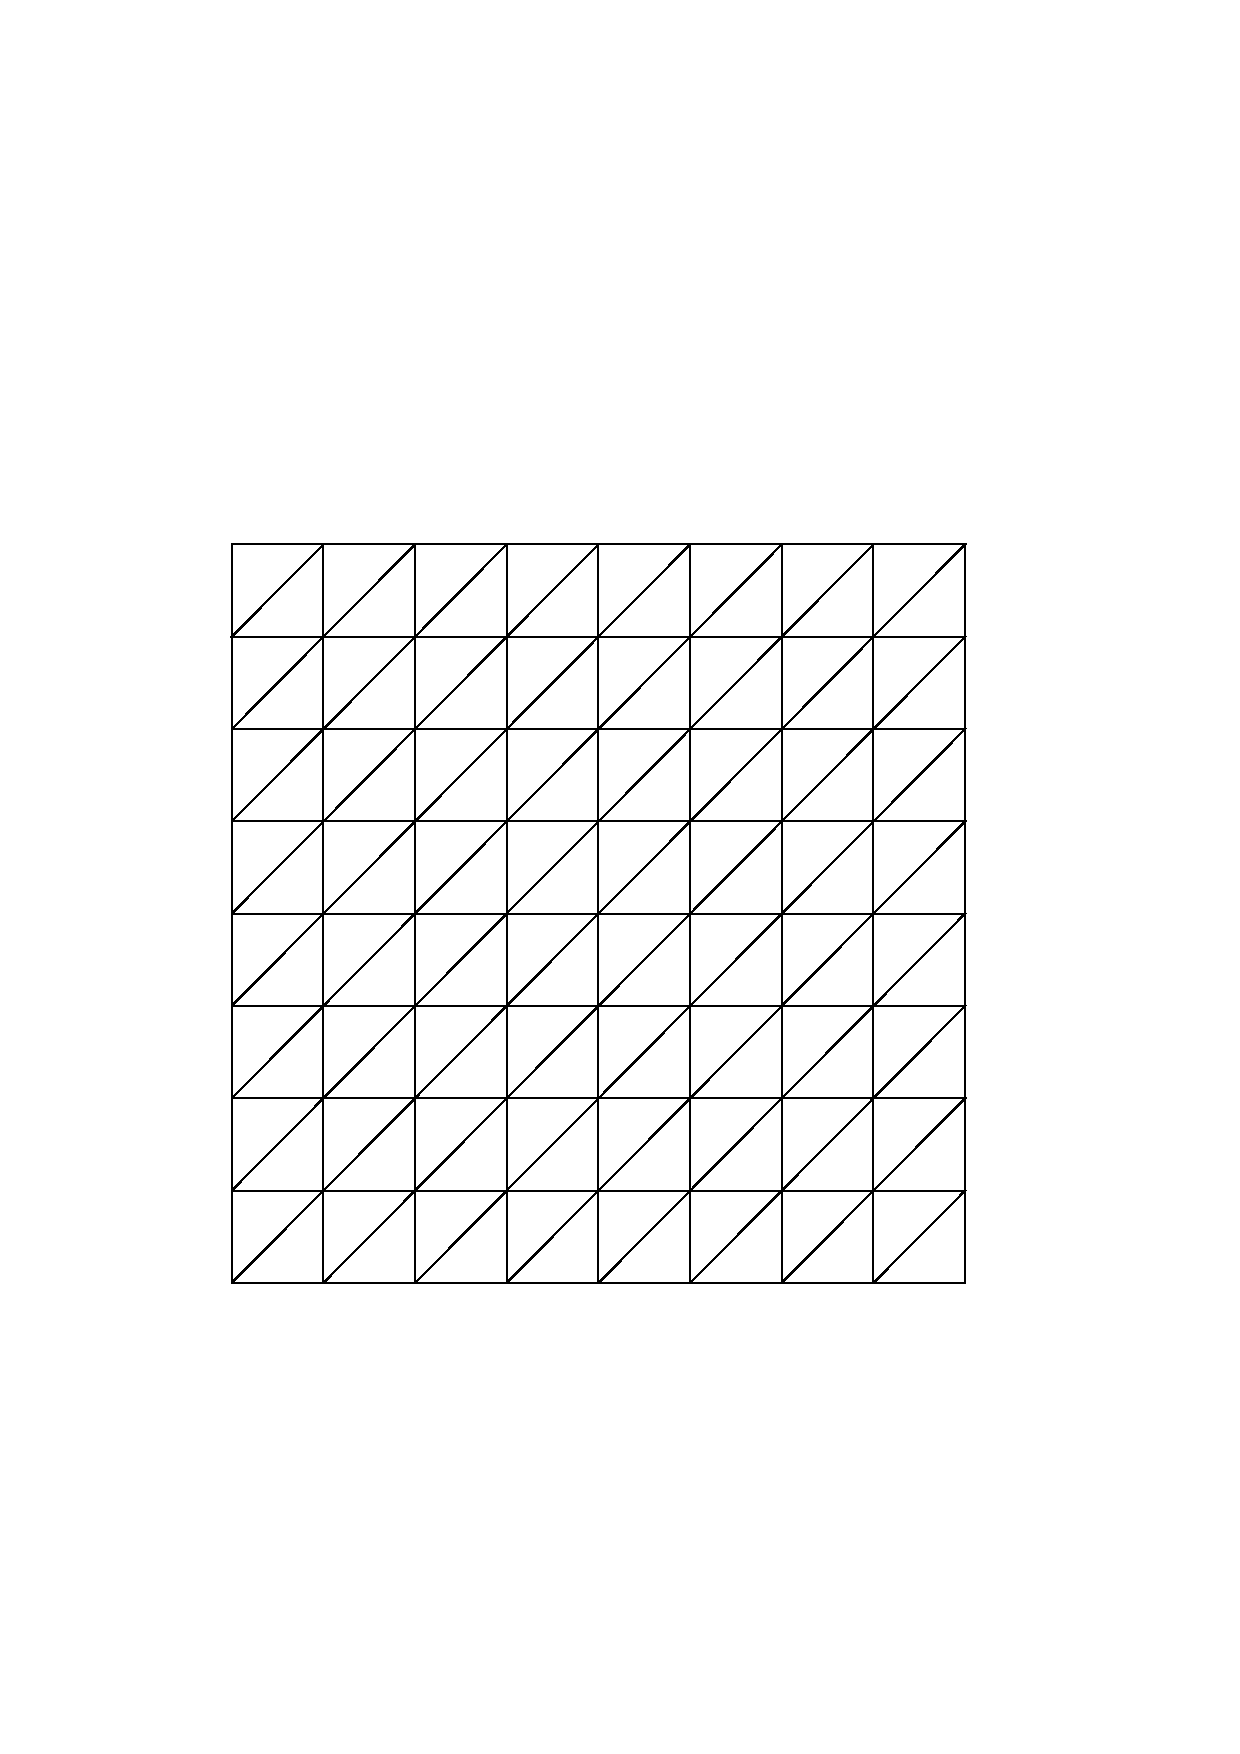
\includegraphics[width=2cm]{figures/grid1.png}
   	 \end{minipage} 
\\\hline
 $\phi_i(x)$   & $\phi_{ij}(x, y)$ 
 \\\hline
 \begin{minipage}{0.4\textwidth}\centering
      	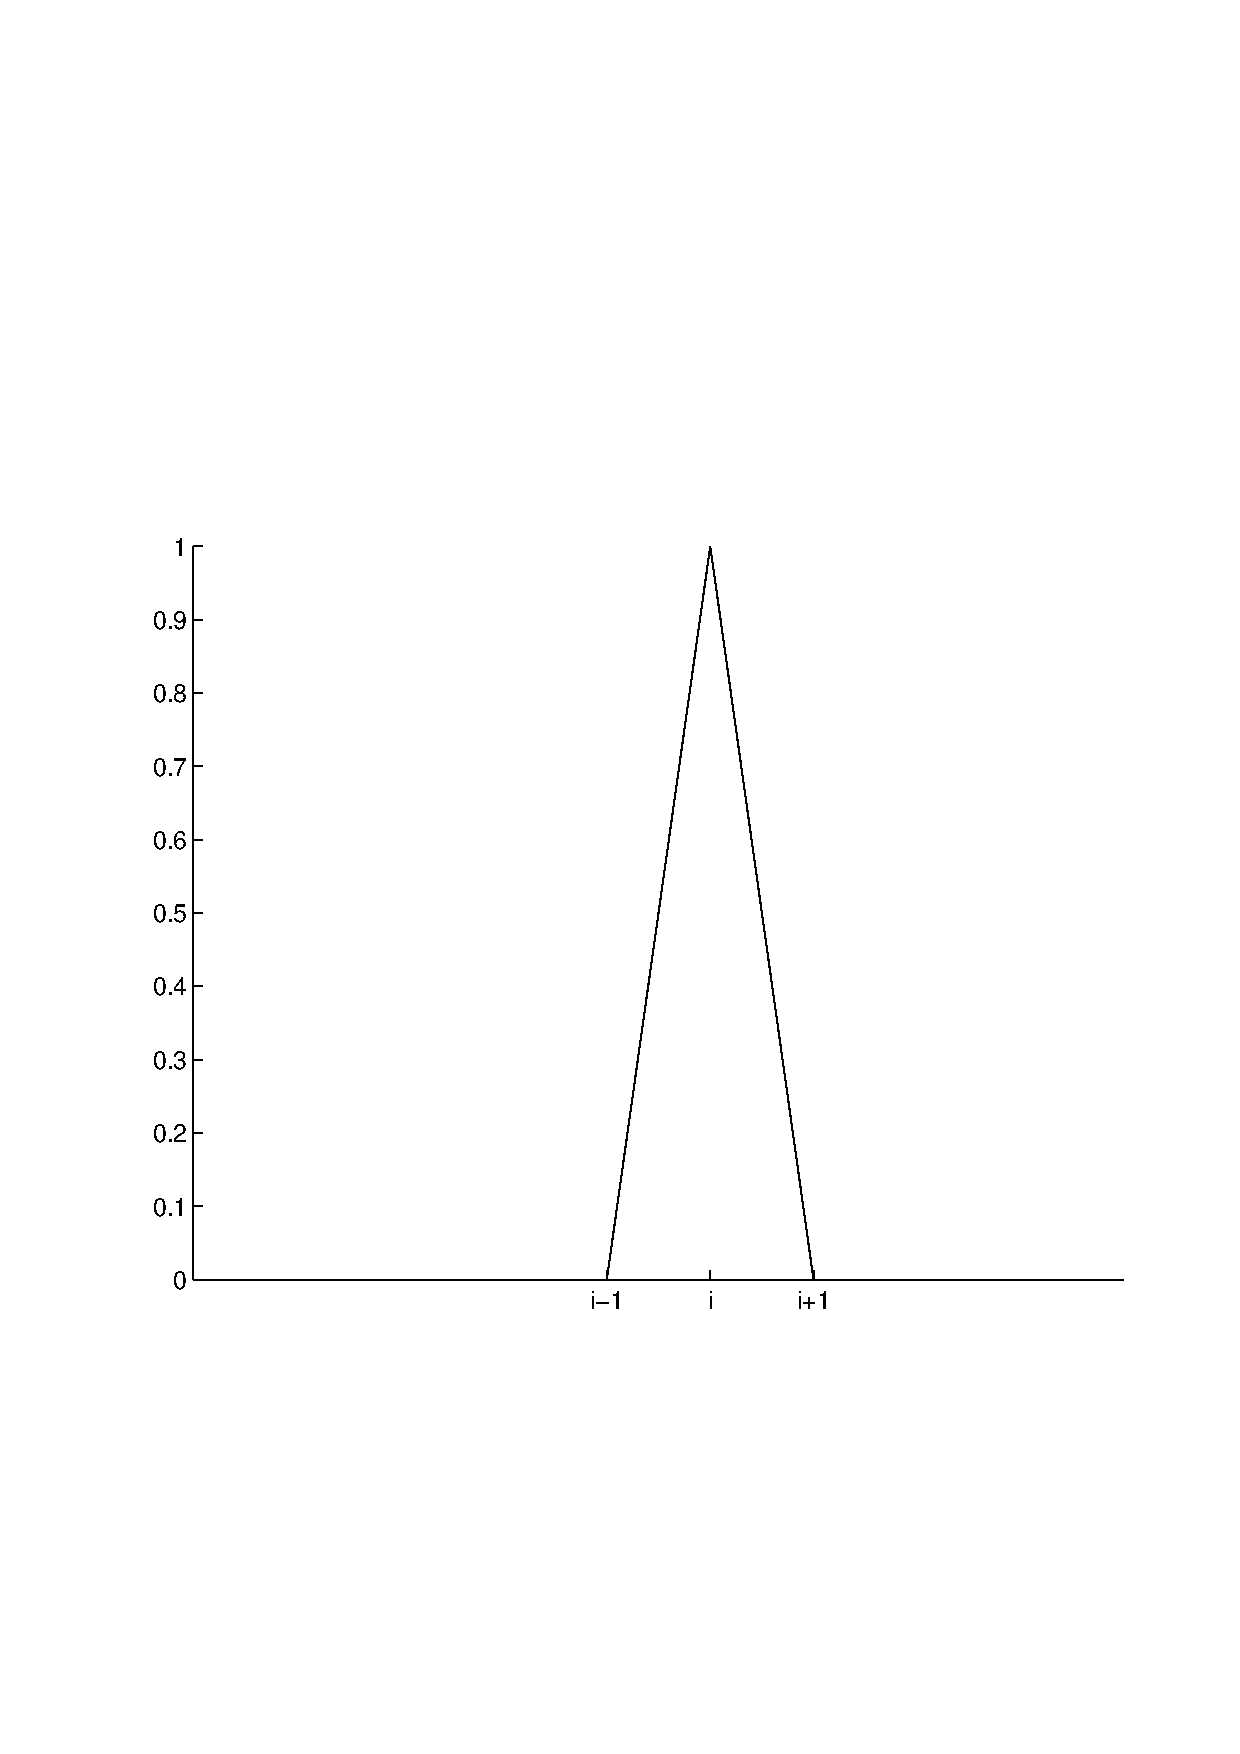
\includegraphics[height=2cm]{figures/basisfunction.pdf}
   	 \end{minipage}
    & \begin{minipage}{0.5\textwidth}\centering
      	\includegraphics[height=2cm]{figures/nodalbasis.pdf}
   	 \end{minipage} 
\\\hline
 \multicolumn{2}{c}{Find $u_h\in V_h$ s.t. $\displaystyle J(u_h)=\min_{v_h\in V_h} J(v_h)$}    
 \\\hline
 $\displaystyle u_h=\sum_{i=1}^n \mu_i\phi_i(x)$         &    $\displaystyle u_h=\sum_{i, j=1}^n \mu_{ij}\phi_{ij}(x, y)$      
  \\\hline
 Find $\mu\in \mathbb{R}^n$ s.t. $\displaystyle  I(\mu)=\min_{\nu\in \mathbb{R}^n} I(\nu)$
 &   Find $\mu\in \mathbb{R}^{n\times n}$ s.t. $\displaystyle  I(\mu)=\min_{\nu\in \mathbb{R}^{n\times n}} I(\nu)$  
 \\\hline
 \multicolumn{2}{c}{$I(\nu)={1\over 2}(A\ast \nu, \nu)_{l^2} - (b, v)_{l^2} $}  
 \\\hline
 $A={1\over h}(-1, 2, -1)$        &   
$\scriptsize
 A=\begin{pmatrix}
 0&-1&0\\
 -1&4&-1\\
 0&-1&0
 \end{pmatrix}
$     
 \\\hline
  \multicolumn{2}{c}{$\mu=\argmin I(\nu) \Longleftrightarrow \nabla J(\mu)=A\ast \mu -b=0$}    \\\hline
\multicolumn{2}{c}{ GD Method:   $ \mu^{(m+1)}=\mu^{(m)} -\eta(A\ast \mu^{(m)}-b)$}       
 \\\hline
$\eta={h\over 4}$       &    $\eta={1\over 8}$      \\\hline
\end{tabular}
\end{table}

\renewcommand\arraystretch{2}
\begin{table}[]
\centerline{\bf Basic multigrid components}
\medskip 
\centering
\begin{tabular}{ p{7cm}<{\centering}|p{7cm}<{\centering}}
\hline 
 \begin{minipage}{0.5\textwidth}
      	\includegraphics[width=7cm,height=3.5cm]{figures/two-grids1.png}
   	 \end{minipage}
    & \begin{minipage}{0.5\textwidth}
      	\includegraphics[width=7cm,height=7cm]{figures/two-grids2.png}
   	 \end{minipage} 
\\\hline
  $\phi_{i}^{2h}={1\over 2} \phi_{2i-1}^{h} + \phi_{2i}^{h} + {1\over 2} \phi_{2i+1}^{h}$        &     { \small$ \phi_{i,j}^{2h} =\phi_{2i,2j}^{h} 
+\frac{1}{2}\left(\phi_{2i-1,2j-1}^{h} +\phi_{2i+1,2j+1}^{h} \right)
+\frac{1}{2}\left(\phi_{2i-1,2j}^{h} +\phi_{2i,2j-1}^{h} 
+\phi_{2i+1,2j}^{h} +\phi_{2i,2j+1}^{2h} \right)$}
      \\\hline
  \multicolumn{2}{c}{ $\Phi^{2h}=R\ast_2 \Phi^h$  }    \\\hline
 $R=({1\over 2}, 1, {1\over 2})$      &   $R=\begin{pmatrix}
0&{1\over 2}&{1\over 2}\\
{1\over 2}&1&{1\over 2}\\
{1\over 2}&{1\over 2}&0
\end{pmatrix}$       \\\hline
\end{tabular}
\end{table}

\clearpage



